%=========================================================================
% (c) 2011, 2012 Josef Lusticky

\section{Topology and hierarchy}\label{sec:ntp-topology}
NTP uses two different communication modes:
one to one, referred as unicast mode, and one to many, referred as broadcast mode~\cite{rfc5905}.
In unicast communication mode, an NTP client sends requests and an NTP server sends responses.
In broadcast communication mode, the client sends no request
and waits for a broadcast mode message from one or more servers~\cite{rfc5905}.

NTP servers are rated with stratum (plural form strata) number representing their level
in an NTP hierarchy and their possible accuracy~\cite{rfc5905}.
Primary (stratum 1) servers synchronise to the reference clock directly traceable to UTC via
radio, satellite or modem.
The stratum 2 servers synchronise to stratum 1
servers via a hierarchical subnet.
The stratum 3 servers synchronise to stratum 2 servers, and so on.
The maximum stratum is 15, number 16 means unsynchronised server
and higher numbers (up to 255) are reserved~\cite{rfc5905}.
Synchronisation between servers in the same stratum level is also possible.
Figure~\ref{fig:ntp-hierarchy} shows a brief hierarchy of NTP.
\begin{figure}
  \centering
  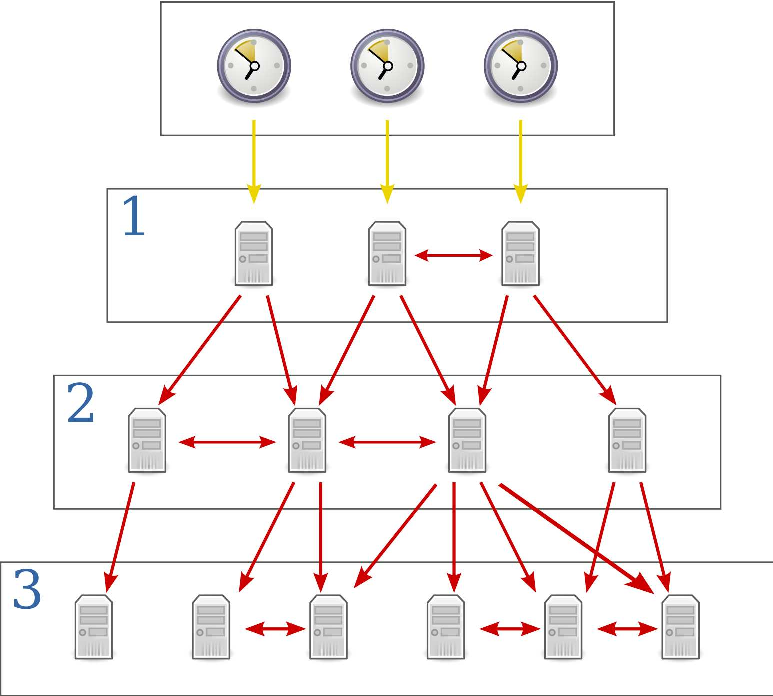
\includegraphics[width=9cm,keepaspectratio]{fig/Network_Time_Protocol_servers_and_clients.pdf}
  \caption{Topology and hierarchy of NTP (source:~\cite{wikimedia-ntp})}
  \label{fig:ntp-hierarchy}
  %\bigskip
\end{figure}
The subnet topology should be organised to avoid timing loops
and minimise synchronisation distances~\cite{rfc5905}.
To achieve this in NTP, the subnet topology is determined using a variant
of the Bellman-Ford distributed routing algorithm, which computes
the shortest-distance spanning tree rooted on the primary (stratum~1) servers~\cite{rfc5905}.
As a result of this design, the
algorithm automatically reorganises the subnet to produce the most accurate and reliable time,
even when one or more primary or secondary servers or the network paths between them fail~\cite{rfc5905}.
